\chapter{Shape Inference}
\label{ch:shape-inference}

So far, we are able to use the shape set
$\mathcal{Y} \subseteq \mathbb{R}^{H \times W \times D} \simeq \mathbb{R}^R$
from Problem \ref{problem} in order to learn a prior model $p(y,z)$ over a
possibly low dimensional latent space $\mathcal{Z} = \mathbb{R}^Q$. To this end,
we introduced variational auto-encoders where the generative model $p(y | z)$ and
the (approximate) recognition model $q(z | y)$ are implemented using
3D convolutional neural networks. In our first approach
to shape completion, we then intend to learn an inference model
\begin{align}
  x \mapsto \tilde{z} \approx &\argmax_{z} p(y = x | z) p(z)\label{eq:shape-inference-amortized-ml}
\end{align}
using a dataset of observations $x \in \mathbb{R}^{H \times W \times D}$.
We call this approach amortized maximum likelihood because we do not consider
the observations $x$ independently, but understand the maximum likelihood objective
as loss allowing to learn the deterministic embedding $x \mapsto \tilde{z}$ in an unsupervised
setting. Given the prior variational auto-encoder, this results in training a
new encoder while keeping the pre-trained decoder fixed.

In the proposed extended variational auto-encoder, we instead understand the
observation $x$ as a random variable. For the corresponding joint distribution
$p(x, y, z)$, we are able to derive the evidence lower bound assuming that
$y$ and $z$ are statistically independent given $x$. Similar to the shape prior,
we learn an approximate recognition model $q(z | x)$ which can be understood
as probabilistic embedding $x \mapsto z$. In contrast to amortized maximum likelihood,
the actual objective tying the observations $x$ to the shapes $y$ is
hidden in a Kullback-Leibler divergence. Again, the model can be trained
in an unsupervised fashion. In addition to training a new encoder, the
extended variational auto-encoder also implements an observation model $p(x | y)$ using a 
3D convolutional neural network. Compared to amortized maximum likelihood,
this potentially allows to explicitly integrate knowledge about the observation model,
however results in longer training time -- also because the embedding $x \mapsto z$
is modeled probabilistically.

In the following, we first discuss a general maximum likelihood approach
to shape completion. Originally, we then experimented with different losses
to learn the embedding $x \mapsto y$ in a non-probabilistic framework. This early
approach is discussed in detail in Appendix \ref{ch:appendix-shape-inference}.
Here, we focus on the proposed amortized maximum likelihood framework which
we discuss using both occupancy grids and signed distance functions
as shape representations. Finally, we consider the proposed extended variational
auto-encoder.

\section{Maximum Likelihood}
\label{sec:shape-inference-maximum-likelihood}

The negative log-likelihood corresponding to Equation
\eqref{eq:shape-inference-amortized-ml} is given by
\begin{align}
  \argmin_{z} - \ln p(y | z) - \ln p(z).\label{eq:shape-inference-nn-ml}
\end{align}
As $p(y | z)$ is a differentiable model,
we can apply gradient descent after decomposing $p(y | z)$ over voxels:
\begin{align}
  - \ln p(y | z) = - \sum_{i = 1}^R \ln p(y_i | z).
\end{align}
where we again flattened the representation of
$y \in \mathbb{R}^{H \times W \times D} \simeq \mathbb{R}^R$.
Considering the actual observations $x_i$, we first discover that
we do not necessarily have an observation $x_i$ for every voxel $i$.
Formally, we write $x \in \{0,1,\uk\}^R$ where $\uk$ indicates
unknown values; in practice, we simply ignore the corresponding indices.
As the probability $p(y_i = x_i | z)$ cannot be determined for $x_i = \uk$,
we exclude them from the optimization problem:
\begin{align}
  \argmin_{z} - \sum_{i = 1, x_i \neq \uk}^R p(y_i | z) - \ln p(z).
\end{align}
As intuition, we assume that the prior $p(z, y)$ is strong enough that
by constraining $p(y | z)$ only for few $y_i$ to specific values (through the
observations $x_i \neq \uk$) will result in good shape predictions.
This is a practical alternative to considering all
$y_i$ with $x_i = \uk$ as hidden variables to optimize in addition to $z$.

% TODO describe somwhere while Gaussian not possible,
% i.e. observed distance function inaccurate
\subsection{Bernoulli Maximum Likelihood}

As mentioned above we assume the observations to be binary, per
voxel. This results in $p(y_i | z)$ being modeled as Bernoulli
distribution. In particular, our generative model predicts
Bernoulli probabilities $\theta_i(z)$ such that
\begin{align}
  p(y_i | z) = \Ber(y_i; \theta_i(z)).
\end{align}
As observations are binary, as well, the probabilities
$p(y_i = x_i | z)$ for $x_i \neq \uk$ can be evaluated directly;
the negative log-likelihood objective can then be written as
loss with respect to $z$:
\begin{align}
  \mathcal{L}_{\text{ML}}(z)
  = - \sum_{i = 1, x_i \neq \uk}^R \ln \Ber(y_i = x_i; \theta_i(z)) - \ln \mathcal{N}(z;0, I_Q)
  \label{eq:shape-inference-ml-loss}
\end{align}
where we also substituted that $p(z)$ is a unit Gaussian in $\mathbb{R}^Q$.
In practice, this simplifies to
\begin{align}
  \mathcal{L}_{\text{ML}}(z)
  = - \sum_{i = 1, x_i \neq \uk}^R (x_i \ln \theta_i(z) + (1 - x_i) \ln (1 - \theta_i(z)))
  + \const + \frac{1}{2}\|z\|^2.
\end{align}
such that the Gaussian prior (\ie $- \ln p(z) \propto \|z\|^2$) represents a
regularizer making sure that the latent code $z$ does not deviate significantly
from the unit Gaussian prior.
We note that this is simply a composite function of the binary cross entropy
error and the sum-of-squared error as introduced in Section \ref{sec:deep-learning-losses}.
% TODO derivative of loss and algorithm?
% TODO similarity to Engelmann

\subsection{Practical Considerations}
\label{sec:shape-inference-ml-practical}

To apply gradient descent to minimize $\mathcal{L}_{\text{ML}}$
we need to be able to compute the gradient $\nabla \mathcal{L}_{\text{ML}}$.
If $\theta_i(z)$ is modeled using a neural network -- as in the case of
variational auto-encoders -- the error backpropagation algorithm can be used.
%In the case of probabilistic PCA, $\theta_i(z)$ is modeled
%by a linear model\footnote{
%  Note that if probabilistic PCA is applied on occupancy grids, we silently
%  re-interpret the reconstructions as occupancy probabilities by
%  clipping them to $[0,1]$ or applying a scaled sigmoid function.
%  We admit that this  does not fit the probabilistic formulation; however,
%  we originally intended to use only signed distance function representations
%  which turns out to be more difficult.
%}. Here, $\theta(z)$ is computed as:
%\begin{align}
%  \theta(z) = g(Uz + \mu) \in \mathbb{R}^R\label{eq:shape-inference-ppca-ml}
%\end{align}
%where $\mu$ is the mean of the shapes $\mathcal{Y}$ and $g$ is a clipping function
%or a scaled sigmoid. The gradient $\nabla \mathcal{L}_{\text{ML}}$ can then
%be computed analogously by error backpropagation, \ie successive application
%of the chain rule. Essentially, Equation \eqref{eq:shape-inference-ppca-ml}
%can be re-interpreted as fully connected layer with bias and non-linearity.
Then, gradient descent with $z^{(0)} = 0$ iteratively performs updates
\begin{align}
  z^{(t + 1)} = z^{(t)} - \gamma \nabla \mathcal{L}_{\text{ML}}(z^{(t)})
\end{align}
where, as discussed earlier, we might adapt the learning rate $\gamma$
over time and also use a momentum parameter. Finally, $z^{(T)}$ 
is used to derive the corresponding shape prediction. We also tried randomly
initializing $z^{(0)}$ and optimizing multiple, different $z^{(0)}$
in parallel but found that this has no significant effect. We additionally
experienced that choosing the learning rate $\gamma$ (as well as the momentum
parameter $\beta$) and the number of iterations $T$ is not trivial
and might vary significantly across observations.
% TODO example with all derivatives, updates for PCA case

\section{Amortized Maximum Likelihood}

% TODO make clear that we are trianing an encoder
% and keeping the decoder
By amortizing, \ie learning, maximum likelihood, we intend to avoid the
optimization problem required for inference in the previous section.
To this end, we introduce a new, deterministic encoder $z(x; w)$
intended to represent the mapping
\begin{align}
  x \mapsto z(x;w) \approx \argmax_{z} p(y = x | z) p(z),
\end{align}
\ie we intend to learn how to directly predict the maximum likelihood solutions.
In practice, the encoder $z(x;w)$ is also implemented using 3D convolutional
neural networks following the architecture of the recognition model $q(z|y)$ from the shape prior.
Using the generative model from the shape-prior, \ie $p(y | z)$,
the encoder $z(x;w)$ can be trained by minimizing a loss derived from the maximum
likelihood formulation. In contrast to the previous section, however,
we also consider the case of signed distance functions as shape representation
where $p(y | z)$ is modeled using Gaussian distributions -- this becomes problematic
when evaluating $p(y_i = x_i | z)$ because $x_i$ is inherently binary (\ie occupied
or not occupied). Overall, this leads to two losses, one for occupancy
derived by assuming Bernoulli distributions and one for signed distance
functions.

\subsection{Bernoulli Amortized Maximum Likelihood}

In the Bernoulli case, the loss reduces to Equation \eqref{eq:shape-inference-ml-loss},
except that the loss is with respect to the parameters $w$ of the new encoder $z(x;w)$:
\begin{align}
  \mathcal{L}&_{\text{AML},\Ber}(w)
  = - \sum_{i = 1, x_i \neq \uk}^R \ln \Ber(y_i = x_i; \theta_i(z)) - \ln \mathcal{N}(z;0, I_Q)\\
  &= - \sum_{i = 1, x_i \neq \uk}^R (x_i \ln \theta_i(z) + (1 - x_i) \ln (1 - \theta_i(z))) + \const + \frac{1}{2}\|z\|^2.
  \label{eq:shape-inference-aml-occ-loss}
\end{align}
where the probabilities $\theta_i(z)$ are predicted by the fixed generative model,
\ie decoder, of the shape prior.
As we are optimizing the parameters $w$, this is equivalent to a binary cross
entropy loss on the observed variables $x_i \neq \uk$ and a quadratic regularizer
on the predicted latent codes $z$.

\subsection{Gaussian Amortized Maximum Likelihood}
\label{sec:shape-inference-gaussian-aml}

\begin{figure}
  \centering
  \hspace*{-0.25cm}
  \begin{subfigure}[t]{0.12\textwidth}
    \includegraphics[height=2cm]{data/2d/input_df/0_output}
  \end{subfigure}
  \begin{subfigure}[t]{0.12\textwidth}
    \includegraphics[height=2cm]{data/2d/input_df/0_input}
  \end{subfigure}
  \begin{subfigure}[t]{0.12\textwidth}
    \includegraphics[height=2cm]{data/2d/input_df/0_space}
  \end{subfigure}
  \begin{subfigure}[t]{0.12\textwidth}
    \includegraphics[height=2cm]{data/2d/input_df/0_output_df}
  \end{subfigure}
  \begin{subfigure}[t]{0.12\textwidth}
    \includegraphics[height=2cm]{data/2d/input_df/0_input_df}
  \end{subfigure}
  \begin{subfigure}[t]{0.12\textwidth}
    \includegraphics[height=2cm]{data/2d/input_df/0_err_space}
  \end{subfigure}\\

  \begin{subfigure}[t]{0.12\textwidth}
    \includegraphics[height=2cm]{data/2d/input_df/2_output}
  \end{subfigure}
  \begin{subfigure}[t]{0.12\textwidth}
    \includegraphics[height=2cm]{data/2d/input_df/2_input}
  \end{subfigure}
  \begin{subfigure}[t]{0.12\textwidth}
    \includegraphics[height=2cm]{data/2d/input_df/2_space}
  \end{subfigure}
  \begin{subfigure}[t]{0.12\textwidth}
    \includegraphics[height=2cm]{data/2d/input_df/2_output_df}
  \end{subfigure}
  \begin{subfigure}[t]{0.12\textwidth}
    \includegraphics[height=2cm]{data/2d/input_df/2_input_df}
  \end{subfigure}
  \begin{subfigure}[t]{0.12\textwidth}
    \includegraphics[height=2cm]{data/2d/input_df/2_err_space}
  \end{subfigure}

  % TODO short caption
  \caption{For implementing the negative log-likelihood $-\ln p(y_i = x_i | z)$
  using Gaussian, \ie continuous, predictions $y_i$, we ca derive (signed) distance
  functions from the given, binary observations $x_i$ for $x_i \neq \uk$ using
  a distance transform.
  %Note that when using real signed distance functions,
  %\ie representing the distance to the original mesh, we would compute
  %the distance to the observed points instead.
  A reasonable loss would then
  compute the negative log-likelihood for all voxels in free space.
  However, in the case of noisy observations,
  even the ground truth shape will have a high negative log-likelihood because
  distance values are affected significantly by few noisy observations.
  To illustrates this phenomenon we show the ground truth shape, the noisy
  observations and the free space in the first three columns for two examples
  from our synthetic 2D dataset, see Appendix \ref{ch:appendix-data}. The
  remaining columns show the distance function of the ground truth shape and
  the noisy observations as well as the the free-space-masked absolute error from
  Equation \eqref{eq:shape-inference-smerr}.}
  \label{fig:shape-inference-sdf-problem}
\end{figure}

When predicting signed distance functions, these are modeled using voxel-wise
Gaussians with fixed variance, \ie
\begin{align}
  p(y_i | z) = \mathcal{N}(y_i;\mu_i(z),\sigma^2).
\end{align}
Ideally, we would derive a signed distance function on our observations
in order to directly use the negative log likelihood $-\ln p(y_i = x_i | z)$ as loss. However,
this leads to a problem illustrated in Figure \ref{fig:shape-inference-sdf-problem}
where the ground truth shape has very high error when defining an absolute error between
the distance function $\text{df}(x_p)$ of observed points $x_p$ and the distance function
$\text{df}(y^*)$ of the ground truth shape $y^*$ when considering voxels in free space only, \ie
\begin{align}
  \sum_{i = 1}^R x_{f,i} \left|\text{df}_i(x_p) - \text{df}_i(y^*)\right|.
  \label{eq:shape-inference-smerr}
\end{align}
Here $x_p$ defines the occupancy grid corresponding to observed points only,
\ie $x_{p,i} = 1$ for $x_i = 1$ and $x_{p,i} = 0$ otherwise.
We also note that $\text{df}(x_p)$ computes, for each voxel, the distance
to the nearest occupied pixel $x_{p,i} = 1$. Similarly, $x_f$
is defined as the occupancy grid corresponding to free space voxels,
\ie $x_{f,i} = 1$ for $x_i = 0$ and $x_{f,i} = 0$ otherwise.
% TODO cite Andreas' paper
Of course, this method of deriving distance functions from the observations
is not ideal; for example, other authors \cite{SteinbrueckerCremers:2013}
compute a distance function along the rays from the observed points. However,
noisy observations are still problematic.%We leave this for future work.

As of the above discussion we would like to use binary observations while still predicting a
shape in signed distance function representation. Then, however, 
evaluating $p(y_i = x_i | z)$ is not meaningful. Instead we need to introduce
a transformation $\theta_i(\mu_i)$ quantifying the probability of occupancy
after having predicted a mean signed distance function value of $\mu_i$.
To this end, we take a closer look on the univariate Gaussian:

% TODO figure of Gaussian and CDF
\begin{figure}
  \centering
  \hspace*{-0.25cm}
  \begin{subfigure}[t]{0.48\textwidth}
    \centering
    \begin{tikzpicture}
      \begin{axis}[
          every axis plot post/.append style={
          mark=none,domain=-3:2,samples=50,smooth},
          axis x line*=bottom,
          axis y line*=left,
          enlargelimits=upper,
          ymax=1.1, ymin=0,
          ylabel=$p(y)$,
          xlabel=$y$,
          legend style={at={(0.65,1)},anchor=north west},
          height=5cm,
          width=7cm,
        ]
      
        \addplot[name path=g,blue] {gauss(-0.75,0.5)};
        \addlegendentry{$p(y)$};
        %\addplot[red] {gauss(1,0.5)};
        %\addlegendentry{$\mu_j(z) = -0.5; \sigma^2 = 0.5$};
        \addplot[blue,dashed,mark=none,forget plot] coordinates {(-0.75, 0) (-0.75, 1)};
        \node at (axis cs:-0.75,1.1) {$\mu_i(z)$};
      
        \addplot[black,dashed,mark=none,forget plot] coordinates {(0, 0) (0, 1)};
        \node at (axis cs:0,1.1) {$0$};
      
        %\addplot[red,dashed,mark=none] coordinates {(1, 0) (1, 0.9)};
        %\node at (axis cs:1,1) {$\mu_j(z)$};
      
        \path[name path=axis] (axis cs:-3,0) -- (axis cs:0,0);
        \addplot [
          thick,
          color=blue,
          fill=blue, 
          fill opacity=0.1,
          area legend, % https://tex.stackexchange.com/questions/246557/custom-area-legend-image-not-working
        ]
        fill between[
          of=g and axis,
          soft clip={domain=-3:0},
        ];
        \addlegendentry{$p(y \leq 0)$}
      \end{axis}
    \end{tikzpicture}
  \end{subfigure}\hfill
  \begin{subfigure}[t]{0.48\textwidth}
    \begin{tikzpicture}
      \begin{axis}[
          every axis plot post/.append style={
          mark=none,domain=-3:2,samples=50,smooth},
          axis x line*=bottom,
          axis y line*=left,
          enlargelimits=upper,
          ymax=1.1, ymin=0,
          ylabel=$p(y' \leq y)$,
          xlabel=$y$,
          legend style={at={(0.65,1)},anchor=north west},
          height=5cm,
          width=7cm,
        ]
      
        % 1.128379167 = 1/(0.5*sqrt(pi))
        \addplot[name path=g,blue] (\x,{0.5*(1 + erf((\x + 0.5)*1.128379167))});
        \addlegendentry{$p(y' \leq y)$};
        \addplot[black,dashed,mark=none,forget plot] coordinates {(0, -1) (0, 1)};
        \node at (axis cs:0,1.1) {$0$};
      \end{axis}
    \end{tikzpicture}
  \end{subfigure}
  %\vskip 6px
  % TODO short caption
  \caption{Illustration of a Gaussian distribution $p(y) = \mathcal{N}(y;-0.75,0.5^2)$
  on the left where the marked area corresponds to the probability $p(y \leq 0)$.
  In our case this refers to the probability of a voxel being occupied. The
  corresponding cumulative density function $p(y' \leq y)$ according to Equation
  \eqref{eq:shape-inference-cdf} is shown on the right.
  }
  \label{fig:shape-inference-gaussian}
\end{figure}

\begin{example}
  As defined in Definition \ref{def:deep-learning-gaussian}, the univariate
  Gaussian distribution takes the form in Figure
  \ref{fig:shape-inference-gaussian}. Its cumulative density
  function is given as
  \begin{align}
    \mathcal{N}(y' \leq y; \mu, \sigma^2) &= \int_{-\infty}^y \mathcal{N}(y'; \mu, \sigma^2) dy'\\
    &= \frac{1}{2}\left(1 + \erf\left(\frac{y - \mu}{\sigma \sqrt{2}}\right)\right).
    \label{eq:shape-inference-cdf}
  \end{align}
  and also shown in Figure \ref{fig:shape-inference-gaussian}.
  The error function $\erf$ is defined as
  \begin{align}
    \erf(y) = \frac{1}{\sqrt{\pi}} \int_{-y}^y \exp(-y'^2) dy'.
  \end{align}
  The cumulative density function quantifies the probability of a variable
  $y'$ falling into a specific range -- in our case $y'$ falling into $(-\infty,y]$.
\end{example}

Using the Gaussian cumulative density function we want to determine the
probability $\theta_i(\mu_i)$ of occupancy.
This process is illustrated in Figure \ref{fig:shape-inference-gaussian};
as negative values in a signed distance function refer to occupied voxels,
we can use
\begin{align}
  \theta_i(\mu_i) &= \mathcal{N}(y' \leq 0; \mu_i, \sigma^2)\\
  &=\frac{1}{2}\left(1 + \erf\left(\frac{- \mu_i}{\sigma \sqrt{\pi}}\right)\right).
  \label{eq:shape-inference-theta-mu-transformation}
\end{align}
Intuitively, we evaluate the cumulative density function at $0$ giving the probability
$\mathcal{N}(y \leq 0; \mu_i(z), \sigma^2)$ which corresponds to the probability of
occupancy. The negative log-likelihood can then be stated as
% TODO theta_i the i is unnecessary
\begin{align}
  \mathcal{L}_{\text{AML},\mathcal{N}}(w) = - \sum_{i = 1,x_i \neq \uk}^R \ln \Ber(y_i = x_i; \theta_i(\mu_i(z))) - \ln \mathcal{N}(z;0,I_Q).
\end{align}
The second term, the negative log-likelihood of the prior $p(z)$ is of course only
added once if the two losses $\mathcal{L}_{\text{AML},\mathcal{N}}$ and
$\mathcal{L}_{\text{AML},\Ber}$ are combined. As before, the negative log-likelihood
of the Bernoulli distributions $\Ber(y_i = x_i; \theta_i(\mu_i(z)))$ leads to the
binary cross entropy error.

\subsection{Practical Considerations}

In practice, we can predict a shape $y$ in both occupancy or signed
distance function representation or use either of them. Compared to
Figure \ref{fig:shape-inference-gaussian}, we generally use a small
variance such as $\ln \sigma^2 = -2 \Leftrightarrow \sigma^2 \approx 0.13533$.
In practice, the fixed variance merely scales the used sum-of-squared loss.
As a result, we found the fixed variance to have negligible impact on training
as long as it is not chosen too small, \eg $\sigma^2 > 0.01$, or too large,
\eg $\sigma^2 < 1$.
Then, for predicting a signed distance function, we add a post-processing layer
which explicitly implements the transformation $\theta(\mu(z))$ from
Equation \eqref{eq:shape-inference-theta-mu-transformation} and allows to
conveniently apply a binary cross entropy loss on top:

\begin{definition}
  A Gaussian to Bernoulli layer $\text{g2b}_{\sigma^2}$ takes as input
  a tensor $\mu \in \mathbb{R}^{B \times C \times H \times W \times D}$ corresponding
  to an element-wise predicted mean (\ie $\mu_i(z)$) of a signed
  distance function and computes a tensor of occupancy probabilities as
  \begin{align}
    (\text{g2b}_{\sigma^2}(\mu))_i &= \int_{-\infty}^0 \mathcal{N}(y_i; \mu_i, \sigma^2) dy_i\\
    &= \frac{1}{2}\left(1 + \erf\left(\frac{-\mu_i}{\sigma \sqrt{\pi}}\right)\right).
  \end{align}
\end{definition}

At this point we note that the derivative of the Gaussian to Bernoulli
layer, which essentially corresponds to the derivative of the Gaussian
cumulative density function, is a Gaussian distribution:
\begin{align}
  \frac{\partial \frac{1}{2}\left(1 + \erf\left(\frac{-\mu_i}{\sigma \sqrt{\pi}}\right)\right)}{\partial \mu_i} &= \left.\frac{\partial \erf(t)}{\partial t}\right|_{t = \frac{-\mu_i}{\sigma\sqrt{\pi}}} \frac{\partial \frac{-\mu_i}{\sigma\sqrt{\pi}}}{\partial \mu_i}\\
  &=\frac{1}{\sqrt{2\pi}\sigma} \exp\left( -\frac{1}{2} \frac{(-\mu_i)^2}{\sigma^2}\right)\\
  &= \mathcal{N}(0; \mu_i, \sigma^2).
\end{align}
The error function $\erf$ is in practice approximated following \cite{Abramowitz:1974}\footnote{
  We use code provided at \url{http://hewgill.com/picomath/lua/erf.lua.html}.
}. If we would additionally predict the variances $\sigma_i^2$, the
derivatives would be more involved, but we did not see any practical benefit of
doing so.
% TODO illustration of training process ... also for non-probabilistic approach!

For both predicting occupancy and signed distance functions,
we found that it is beneficial to weight the prior, \eg
\begin{align}
  \mathcal{L}_{\text{AML}}(w) = - \sum_{i = 1,x_i \neq \uk}^R \ln \Ber(y_i = x_i; \theta_i(z)) - \kappa \ln \mathcal{N}(z;0,I_Q);
  \label{eq:shape-inference-aml-weighted-loss}
\end{align}
especially on datasets with noise, it is important that the encoder
$z(x;w)$ learns to predict latent codes $z$ that are likely under the
unit Gaussian prior $p(z)$. This prevents the encoder from getting distracted
by noise which usually also leads to unlikely codes $z$.

\section{Extended Variational Auto-Encoder}

% TODO plate notation M,N or R/Q?
\begin{figure}
  \centering
  \hspace*{-0.5cm}
  \begin{subfigure}[t]{0.48\textwidth}
    \centering
    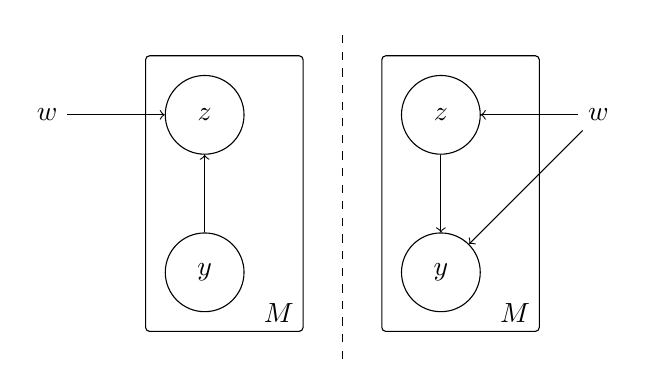
\begin{tikzpicture}

      \node[rectangle,rounded corners=0.05cm,draw=black,minimum width=2cm,minimum height=3.5cm] (M) at (0.25, -1){};
      \node[above left] at (M.south east){$M$};
      \node[circle,draw=black,minimum size=1cm] (z) at (0,0){$z$};
      \node[circle,draw=black,minimum size=1cm] (y) at (0,-2){$y$};
      \node[] (w) at (-2,0){$w$};
      
      \draw[->] (w) -- (z);
      \draw[->] (y) -- (z);
      
      \draw[-,dashed] (1.75,-3.1) -- (1.75,1.1);
      
      \node[rectangle,rounded corners=0.05cm,draw=black,minimum width=2cm,minimum height=3.5cm] (M) at (3.25, -1){};
      \node[above left] at (M.south east){$M$};
      \node[circle,draw=black,minimum size=1cm] (z) at (3,0){$z$};
      \node[circle,draw=black,minimum size=1cm] (y) at (3,-2){$y$};
      \node[] (w) at (5,0){$w$};
      
      \draw[->] (w) -- (z);
      \draw[->] (w) -- (y);
      \draw[->] (z) -- (y);
      
    \end{tikzpicture}
    \vskip 6px
    \caption{Illustration of the graphical model of the original variational
    auto-encoder as discussed in Chapter \ref{ch:shape-prior}.
    The generative model is shown on the right and governed by $p(y, z) = p(y|z)p(z)$,
    while the recognition model is shown on the left and
    approximated by $q(z|y)$.}
    \label{subfig:shape-inference-vae}
  \end{subfigure}\hfill
  \begin{subfigure}[t]{0.48\textwidth}
    \centering
    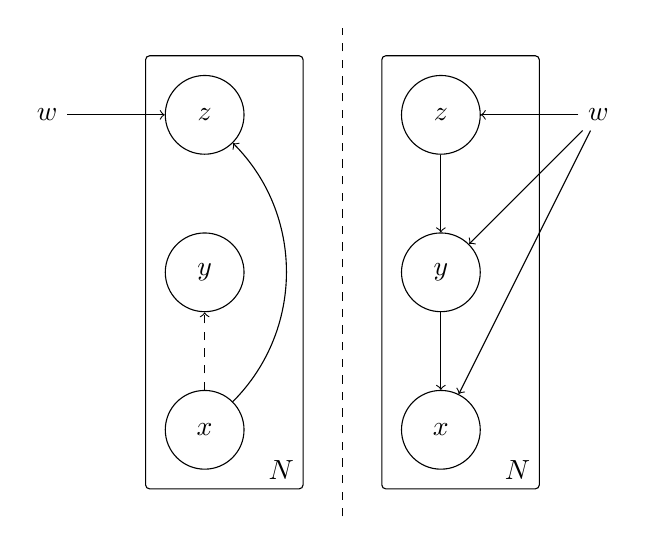
\begin{tikzpicture}

      \node[rectangle,rounded corners=0.05cm,draw=black,minimum width=2cm,minimum height=5.5cm] (M) at (0.25, -2){};
      \node[above left] at (M.south east){$N$};
      \node[circle,draw=black,minimum size=1cm] (z) at (0,0){$z$};
      \node[circle,draw=black,minimum size=1cm] (y) at (0,-2){$y$};
      \node[circle,draw=black,minimum size=1cm] (x) at (0,-4){$x$};
      \node[] (w) at (-2,0){$w$};
      
      \draw[->] (w) -- (z);
      %\draw[->] (y) -- (z);
      \draw[->,dashed] (x) -- (y);
      \draw[->] (x) to [out=45,in=315](z);
      
      \draw[-,dashed] (1.75,-5.1) -- (1.75,1.1);
      
      \node[rectangle,rounded corners=0.05cm,draw=black,minimum width=2cm,minimum height=5.5cm] (M) at (3.25, -2){};
      \node[above left] at (M.south east){$N$};
      \node[circle,draw=black,minimum size=1cm] (z) at (3,0){$z$};
      \node[circle,draw=black,minimum size=1cm] (y) at (3,-2){$y$};
      \node[circle,draw=black,minimum size=1cm] (x) at (3,-4){$x$};
      \node[] (w) at (5,0){$w$};
      
      \draw[->] (w) -- (z);
      \draw[->] (w) -- (y);
      \draw[->] (w) -- (x);
      \draw[->] (z) -- (y);
      \draw[->] (y) -- (x);

    \end{tikzpicture}
    \vskip 6px
    % TODO text model
    \caption{Illustration of the graphical model of the extended
  variational auto-encoder explicitly taking into account the observation $x$.
  The generative model on the right assumes that first a shape $y$
  is generated through $p(y | z)$ and the observation $x$ is then
  obtained from the observation model $p(x | y)$. In the inference model on
  the left the latent code $z$ is inferred through $q(z | x)$ -- this can be
  seen as probabilistic embedding of observation $x$ in the latent shape space.
  The (dashed) model $q(y | x)$ is not learned but used to tie the observation $x$
  to the predicted shape $y$.}
    \label{subfig:shape-inference-evae}
  \end{subfigure}
  \vskip 6px
  % TODO short caption
  \caption{Comparison of the regular variational auto-encoder model in Figure
  \ref{subfig:shape-inference-vae} to learn a shape prior and the 
  extended variational auto-encoder model to learn shape completion in
  Figure \ref{subfig:shape-inference-evae}.}
  \label{fig:shape-inference}
\end{figure}

The approaches discussed above are formulated in a maximum likelihood framework
where we consider $x_i$ to be actual observations of the random variables $y_i$. In contrast,
we might also directly extend the graphical model in Figure \ref{subfig:shape-inference-vae}
to also consider the observation $x_i$ as random variable.
In Figure \ref{subfig:shape-inference-evae}
we illustrate a possible extension that we decided to investigate closer.
The main idea is to model the observation process $p(x | y)$ explicitly in order
to deduce information about a possible $y$. There are many possibilities to
model $p(x | y)$ -- \eg by learning it directly from samples $\{(x_n, y_n^*)\}$
or by modeling the sensor. Here, we leave these options for future work
and model $p(x | y)$ through a neural network without direct supervision
by embedding $p(x | y)$ in the framework of variational inference.

Following the introduction of variational inference in Section \ref{sec:variational-inference},
the evidence lower bound for the model in Figure \ref{subfig:shape-inference-evae} can be
written as
\begin{align}
  - \text{KL}(q(y,z|x)|p(y,z)) + \mathbb{E}_{q(y,z|x)}[\ln p(x|y)]
\end{align}
This formulation treats both $y$ and $z$ as latent variables regarding the
newly introduced random variable $x$. The exact structure of $q(y,z|x)$ as well
as $p(y,z)$ is not defined yet. For the latter we again use a pre-trained shape prior
$p(y,z) = p(y|z) p(z)$; for the former we have to make simplifying assumptions.
In particular, we assume that $y$ and $z$ are statistically independent given $x$:
\begin{align}
  q(y, z | x) = q(y | x) q(z | x).
\end{align}
Here, $q(z | x)$ is the mapping we want to learn; $p(y | x)$ decomposes into
\begin{align}
  q(y | x) = \prod_{i = 1}^R q(y_i | x_i)
\end{align}
and can easily be modeled for those voxels $x_i$ where we have observations, \ie
$x_i \neq \uk$. Note that $q(y | x)$ is not learned, \ie it is
not modeled through a neural network -- it is not part of the recognition model;
however $q(y | x)$ allows us to integrate
knowledge about the observations within the Kullback-Leibler divergence:
\begin{align}
  \text{KL}(q(y,z|x)|p(y,z)) &= \mathbb{E}_{q(y, z | x)}\left[\ln\frac{q(y, z | x)}{p(y, z)}\right]\\
  &= \mathbb{E}_{q(y, z | x)}\left[\ln\frac{q(y | x)q(z | x)}{p(y | z)p(y)}\right]\\
  &= \mathbb{E}_{q(y | x)}\left[\ln\frac{q(y | x)}{p(y | z)}\right] + \mathbb{E}_{q(z | x)}\left[\ln\frac{q(z | x)}{p(z)}\right]\\
  &= \KL(q(y|x) | p(y|z)) + \KL(q(z|x)|p(z))
\end{align}
Finally, the reconstruction error simplifies to
\begin{align}
  \mathbb{E}_{q(y,z|x)}[\ln p(x|y)] = \mathbb{E}_{q(y|x)}[\ln p(x|y)].
\end{align}
Then, the overall objective can then be written as
\begin{align}
  \mathcal{L}_{\text{EVAE}}(w) = \text{KL}(q(z | x)|p(z)) + \text{KL}(q(y | x)|p(y | z)) 
  - \mathbb{E}_{q(y | x)}[\ln p(x | y)]
  \label{eq:shape-inference-evae}
\end{align}
where the Kullback-Leibler divergence $\text{KL}(q(y | x)|p(y | z))$ implicitly
ties the observation $x$ to the possible shape $y$.

% TODO introduce concept of Monte Carlo samples
As before, both Kullback-Leibler divergences can be computed analytically. Only
the reconstruction error $\mathbb{E}_{q(y|x)}[\ln p(x|y)]$ needs to be 
approximated using Monte-Carlo samples; for a specific sample $x_n$, this means
\begin{align}
  - \mathbb{E}_{q(y | x)}[\ln p(x | y)] = - \sum_{l = 1}^L \ln p(x_n | y_{l,n})
\end{align}
% TODO multiariate uniform distribution ...
with
\begin{align}
  y_{l,n} &= g_y(z_{l,n}, \epsilon_{l,n})\quad\text{ and }\quad\epsilon_{l,n} \sim U(0,1)^R\\
  z_{l,n} &= g_z(x_n, \epsilon'_{l,n})\quad\text{ and }\quad\epsilon'_{l,n} \sim \mathcal{N}(\epsilon;0,I_Q)
\end{align}
and usually using $L = 1$ sample. Here, $g_y$ represents the Bernoulli
reparameterization trick from
Section \ref{sec:shape-prior-bernoulli-vae} and $g_z$ the Gaussian equivalent
from Section \ref{sec:shape-prior-gaussian-vae}. This also implies that
$y_i$ is modeled using a Bernoulli distribution, just like $x_i$, while
$z$ is modeled using a Gaussian distribution. To make this explicit,
we write
% TODO theta and rho?
\begin{align}
  p(z) &= \mathcal{N}(z;\mu(x), \diag(\sigma^2(x)))\\
  p(y_i | z) &= \Ber(y_i;\theta_i(z))\\
  p(x_i | y) &= \Ber(x_i;\rho_i(y))
\end{align}
where the parameters $\mu$, $\sigma^2$ as well as $\theta_i$, $\rho_i$
are modeled using neural networks; in particular, $\theta_i(z)$ is taken
from the pre-trained shape prior in order to restrict shape inference to
reasonable shapes. Overall,
this specifies the generative model of the extended variational auto-encoder
as in Figure \ref{subfig:shape-inference-evae} on the right.

In Equation \eqref{eq:shape-inference-evae}, only the Kullback-Leibler divergence
$\KL(q(y|x)|p(y|z))$ as well as the recognition model $q(z|x)$ are left
for discussion. The approximate posterior $q(z|x)$ is modeled analogously
to $q(z|y)$. For the Kullback-Leibler divergence, we follow the
maximum likelihood formulation and use:
\begin{align}
  q(y_i | x_i = 1) &= \Ber(y_i; 1)\\
  q(y_i | x_i = 0) &= \Ber(y_i; 0)
\end{align}
while ignoring unobserved voxels $x_i = \uk$ as we assume a strong enough 
shape prior that is able to fill in the unobserved voxels.
The Kullback-Leibler divergence $\KL(q(y|x)|p(y|z))$ then implicitly tries to
adjust the predicted shape $y$ to the observation $x$.

\subsection{Practical Considerations}

% TODO implementation details with figure
We already introduced all the necessary
tools for implementing the proposed model in Chapter \ref{ch:shape-prior}.
The latent code $z$ is still modeled as Gaussian;
so, for the Kullback-Leibler divergence $\KL(q(z|x) | p(z))$ Equation
\eqref{eq:shape-prior-analyitcal-kld} applies:
\begin{align}
  \KL(q(z|x) | p(z)) &= \sum_{i = 1}^Q \KL(\mathcal{N}(z_i; \mu_i(x), \sigma_i(x)^2) | \mathcal{N}(z_i; 0, 1))\\
  &= \sum_{i = 1}^Q \left(- \frac{1}{2} \ln \sigma_i(x) + \frac{1}{2} \sigma_i(x)^2 + \frac{1}{2} \mu_i^2(x) - \frac{1}{2}\right).
\end{align}
The voxels $y_i$ are modeled using Bernoulli distributions and $p(y|z)$
is taken from the shape prior; it is not fine-tuned but
kept fixed. The Kullback-Leibler divergence $\KL(q(y|x)|p(y|z))$ 
follows Equation \eqref{eq:shape-prior-bernoulli-kld} and can be written as
\begin{align}
  \KL(q(y&|x)|p(y|z)) = \sum_{i = 1}^R \KL(q(y_i|x_i)|p(y_i|z))\\
  &= \sum_{i = 1, x_i \neq \uk}^R \sum_{k \in \{0,1\}} \left.\begin{cases}
    \ln 1^k 0^{1 - k} & \quad x_i = 1\\
    \ln 0^k 1^{1 - k} & \quad x_i = 0
  \end{cases}\right\} - \ln \theta_i(z)^k (1 - \theta_i(z))^{1-k}.
  \label{eq:shape-inference-evae-kld}
\end{align}
In practice, for numerical reasons, we need to add a small $\epsilon$-term
to avoid taking the natural logarithm $\ln 0$, \ie $\ln \theta^k (1-\theta)^k$
becomes $\ln (\theta + \epsilon)^k (1 - \theta + \epsilon)^{1 - k}$.
The pre-trained generative model $p(y | z)$ is then followed by a Bernoulli
Kullback-Leibler layer (\cf Definition \ref{def:shape-prior-bernoulli-kld})
implementing Equation \eqref{eq:shape-inference-evae-kld}
and a Bernoulli reparameterization layer (\cf Definition \ref{def:shape-prior-bernoulli-repa}).
The observation model $p(x | y)$ is then learned using a 3D convolutional neural
network as illustrated in Figure \ref{fig:shape-inference-evae}.
% TODO example

% TODO light gray, surround the individual parts, i.e.
% q(z|x), p(y|z) and p(x|y)
%\begin{figure}
%  \centering
%  \begin{tikzpicture}
%    \node (x) at (0,0) {$x$};
%
%    \node[conv,rotate=90,minimum width=4cm] (conv1) at (1.25,0) {$\text{conv}_{1, C_1, K}$ + $\text{bn}$ + $h$};
%    \node[pool,rotate=90,minimum width=4cm] (pool1) at (2.5,0) {$\text{pool}_{2}$};
%    \node[conv,rotate=90,minimum width=4cm] (conv2) at (3.75,0) {$\text{conv}_{C_1, C_2, K}$ + $\text{bn}$ + $h$};
%    \node[pool,rotate=90,minimum width=4cm] (pool2) at (5,0) {$\text{pool}_{2}$};
%    \node[view,rotate=90,minimum width=4cm] (view2) at (6.25,0) {$\text{view}_{B, C_3}$};
%    
%    \node[fc,rotate=90, minimum width = 1.8625cm] (fc21) at (8,1.07525) {$\text{fc}_{C_3, Q}$};
%    \node[fc,rotate=90, minimum width = 1.8625cm] (fc22) at (8,-1.07525) {$\text{fc}_{C_3, Q}$};
%  
%    \node at (9, 1.15){$\mu$};
%    \node at (9, -1.15){$\sigma^2$};
%  
%    \node[view,rotate=90,minimum width=4cm] (kld1) at (10,0) {$\text{KLD}_{\mathcal{N}}$};
%    \node[view,rotate=90,minimum width=4cm] (repa1) at (12,0) {$\text{repa}_{\mathcal{N}}$};
%    
%    \node at (11,0.3){$\mu,\sigma^2$};
%    
%    \node (z) at (13.5,-2.5){$z$};
%    
%    \node[fc,rotate=90,minimum width=4cm] (fc3) at (12,-5) {$\text{fc}_{Q, C_3}$};
%    \node[view,rotate=90,minimum width=4cm] (view3) at (10.75,-5) {$\text{view}_{B, C_2, \floor{\frac{H}{4}}, \floor{\frac{W}{4}}, \floor{\frac{D}{4}}}$};
%    
%    \node[up,rotate=90,minimum width=4cm] (up4) at (9.5,-5) {$\text{nnup}_{2}$};
%    \node[conv,rotate=90,minimum width=4cm] (conv4) at (8.25,-5) {$\text{conv}_{C_2, C_1, K}$ + $\text{bn}$ + $h$};
%    
%    \node[up,rotate=90,minimum width=4cm] (up5) at (7,-5) {$\text{nnup}_{2}$};
%    \node[conv,rotate=90,minimum width=4cm] (conv5) at (5.75,-5) {$\text{conv}_{C_1, 1, K}$ + $\text{bn}$ + $h$};
%    
%    \node at (4.75,-4.7){$\theta$};
%    
%    \node[view,rotate=90,minimum width=4cm] (kld2) at (3.75,-5) {$\text{KLD}_{\Ber}$};
%    
%    \node at (2.75,-4.7){$\theta$};
%    
%    \node[view,rotate=90,minimum width=4cm] (repa2) at (1.75,-5) {$\text{repa}_{\Ber}$};
%    
%    \node (y) at (0,-7.5) {$\tilde{y}$};
%    
%    \node[conv,rotate=90,minimum width=4cm] (conv6) at (1.25,-10) {$\text{conv}_{1, C_4, K}$ + $\text{bn}$ + $h$};
%    \node[conv,rotate=90,minimum width=4cm] (conv7) at (2.5,-10) {$\text{conv}_{C_4, C_5, K}$ + $\text{bn}$ + $h$};
%    \node[conv,rotate=90,minimum width=4cm] (conv8) at (3.75,-10) {$\text{conv}_{C_5, C_1, K}$ + $\text{bn}$ + $h$};
%    
%    \node (rx) at (13.5, -10) {$\tilde{x}$};
%    
%    \draw[->] (x) -- (conv1);
%    \draw[->] (conv1) -- (pool1);
%    \draw[->] (pool1) -- (conv2);
%    \draw[->] (conv2) -- (pool2);
%    \draw[->] (pool2) -- (view2);
%    \draw[->] (view2) -- (fc21);
%    \draw[->] (view2) -- (fc22);
%    \draw[->] (fc21) -- (kld1);
%    \draw[->] (fc22) -- (kld1);
%    \draw[->] (kld) -- (repa1);
%    \draw[-] (repa1) -- (13.5,0);
%    \draw[->] (13.5,0) -- (z);
%    \draw[-] (z) -- (13.5,-5);
%    \draw[->] (13.5,-5) -- (fc3);
%    \draw[->] (fc3) -- (view3);
%    \draw[->] (view3) -- (up4);
%    \draw[->] (up4) -- (conv4);
%    \draw[->] (conv4) -- (up5);
%    \draw[->] (up5) -- (conv5);
%    \draw[->] (conv5) -- (kld2);
%    \draw[->] (kld2) -- (repa2);
%    \draw[-] (repa2) -- (0,-5);
%    \draw[->] (0,-5) -- (y);
%    \draw[-] (y) -- (0,-10);
%    \draw[->] (0,-10) -- (conv6);
%    \draw[->] (conv6) -- (conv7);
%    \draw[->] (conv7) -- (conv8);
%    \draw[->] (conv8) -- (rx);
%  \end{tikzpicture}
%  \vskip 6px
%  
%  \caption{Illustration of the extended variational auto-encoder. For
%  comparison, we also consider Figure \ref{fig:shape-prior-variational-auto-encoder}
%  of the standard variational auto-encoder. Here, both $q(z|x)$ and $p(y|z)$
%  are represented by convolutional neural networks mirroring each other;
%  each consisting of two stages of convolutional layers including batch normalization,
%  non-linearity and pooling.
%  The decoder, \ie $p(y|z)$, is kept fixed after pre-training; the encoder
%  $q(z|x)$ is either trained from scratch or fine-tuned from $q(z|y)$.
%  The last part, the convolutional neural network modeling $p(x|y)$, consists
%  of three stages of convolutional layers including batch normalization and non-linearity.
%  Here, no pooling layers can be found as the size of the output $x$
%  matches the size of its input $y$.}
%  \label{fig:shape-inference-evae}
%\end{figure}

\begin{figure}
  \centering
  \hspace*{-0.75cm}
  \begin{tikzpicture}
    \node (x) at (0,0) {\small$x$};

    \node[conv,rotate=90,minimum width=4.5cm] (conv1) at (2.5,0) {\small$\text{conv}_{1, 16, 3}$\,+\,$\text{bn}$\,+\,$\ReLU$};
    \node[pool,rotate=90,minimum width=4.5cm] (pool1) at (3.75,0) {\small$\text{pool}_{2}$};
    \node[conv,rotate=90,minimum width=4.5cm] (conv2) at (5,0) {\small$\text{conv}_{16, 32, 3}$\,+\,$\text{bn}$\,+\,$\ReLU$};
    \node[pool,rotate=90,minimum width=4.5cm] (pool2) at (6.25,0) {\small$\text{pool}_{2}$};
    \node[conv,rotate=90,minimum width=4.5cm] (conv3) at (7.5,0) {\small$\text{conv}_{32, 64, 3}$\,+\,$\text{bn}$\,+\,$\ReLU$};
    \node[pool,rotate=90,minimum width=4.5cm] (pool3) at (8.75,0) {\small$\text{pool}_{2}$};
    \node[conv,rotate=90,minimum width=4.5cm] (conv4) at (10,0) {\small$\text{conv}_{64, 128, 3}$\,+\,$\text{bn}$\,+\,$\ReLU$};
    \node[pool,rotate=90,minimum width=4.5cm] (pool4) at (11.25,0) {\small$\text{pool}_{2}$};
    
    \node[view,rotate=90,minimum width=4.5cm] (view4) at (12.5,0) {\small$\text{view}_{B, 1024}$};
    
    \node[fc,rotate=90, minimum width = 2cm] (fc51) at (13.75,1.25) {\small$\text{fc}_{512, Q}$};
    \node[fc,rotate=90, minimum width = 2cm] (fc52) at (13.75,-1.25) {\small$\text{fc}_{512, Q}$};
  
    \node[view,rotate=90,minimum width=4.5cm] (kld) at (15,0) {\small$\text{KLD}_{\mathcal{N}}$\,+\,$\text{repa}_{\mathcal{N}}$};
    
    \node (z) at (15,-5){\small$\tilde{z}$};
    
    \node[fc,rotate=90,minimum width=4.5cm] (fc6) at (13.75,-5) {\small$\text{fc}_{Q, 512}$};
    \node[view,rotate=90,minimum width=4.5cm] (view6) at (12.5,-5) {\small$\text{view}_{B, 1024, 2, 2, 2}$};
    
    \node[up,rotate=90,minimum width=4.5cm] (up7) at (11.25,-5) {\small$\text{nnup}_{2}$};
    \node[conv,rotate=90,minimum width=4.5cm] (conv7) at (10,-5) {\small$\text{conv}_{128, 64, 3}$\,+\,$\text{bn}$\,+\,$\ReLU$};
    \node[up,rotate=90,minimum width=4.5cm] (up8) at (8.75,-5) {\small$\text{nnup}_{2}$};
    \node[conv,rotate=90,minimum width=4.5cm] (conv8) at (7.5,-5) {\small$\text{conv}_{64, 32, 3}$\,+\,$\text{bn}$\,+\,$\ReLU$};
    \node[up,rotate=90,minimum width=4.5cm] (up9) at (6.25,-5) {\small$\text{nnup}_{2}$};
    \node[conv,rotate=90,minimum width=4.5cm] (conv9) at (5,-5) {\small$\text{conv}_{32, 16, 3}$\,+\,$\text{bn}$\,+\,$\ReLU$};
    \node[up,rotate=90,minimum width=4.5cm] (up10) at (3.75,-5) {\small$\text{nnup}_{2}$};
    \node[conv,rotate=90,minimum width=4.5cm] (conv10) at (2.5,-5) {\small$\text{conv}_{16, 1, 3}$\,+\,$\text{bn}$\,+\,$h$};
    
    \node[view,rotate=90,minimum width=4.5cm] (kld2) at (1.25,-5) {\small$\text{KLD}_{\Ber}$\,+\,$\text{repa}_{\Ber}$\,+\,$\sigma$};
    \node (ry) at (0,-5) {\small$\tilde{y}$};
    
    \node[conv,rotate=90,minimum width=4.5cm] (conv11) at (1.25,-10) {\small$\text{conv}_{1, 16, 3}$\,+\,$\text{bn}$\,+\,$\ReLU$};
    \node[conv,rotate=90,minimum width=4.5cm] (conv12) at (2.5,-10) {\small$\text{conv}_{16, 32, 3}$\,+\,$\text{bn}$ + $\ReLU$};
    \node[conv,rotate=90,minimum width=4.5cm] (conv13) at (3.75,-10) {\small$\text{conv}_{32, 64, 3}$\,+\,$\text{bn}$\,+\,$\ReLU$};
    \node[conv,rotate=90,minimum width=4.5cm] (conv14) at (5,-10) {\small$\text{conv}_{64, 128, 3}$\,+\,$\text{bn}$\,+\,$\ReLU$};
    \node[conv,rotate=90,minimum width=4.5cm] (conv15) at (6.25,-10) {\small$\text{conv}_{128, 64, 3}$\,+\,$\text{bn}$\,+\,$\ReLU$};
    \node[conv,rotate=90,minimum width=4.5cm] (conv16) at (7.5,-10) {\small$\text{conv}_{64, 32, 3}$\,+\,$\text{bn}$\,+\,$\ReLU$};
    \node[conv,rotate=90,minimum width=4.5cm] (conv17) at (8.74,-10) {\small$\text{conv}_{32, 16, 3}$\,+\,$\text{bn}$\,+\,$\ReLU$};
    \node[conv,rotate=90,minimum width=4.5cm] (conv18) at (10,-10) {\small$\text{conv}_{16, 1, 3}$\,+\,$\text{bn}$\,+\,$\sigma$};
    
    \node (rx) at (15, -10) {\small$\tilde{x}$};
    
    \draw[->] (y) -- (conv1);
    \draw[->] (conv1) -- (pool1);
    \draw[->] (pool1) -- (conv2);
    
    \draw[->] (conv2) -- (pool2);
    \draw[->] (pool2) -- (conv3);
    
    \draw[->] (conv3) -- (pool3);
    \draw[->] (pool3) -- (conv4);
    
    \draw[->] (conv4) -- (pool4);
    \draw[->] (pool4) -- (view4);
    
    \draw[->] (view4) -- (fc51);
    \draw[->] (view4) -- (fc52);
    
    \draw[->] (fc51) -- (kld);
    \draw[->] (fc52) -- (kld);
    
    \draw[->] (kld) -- (z);
    \draw[->] (z) -- (fc6);
    \draw[->] (fc6) -- (view6);
    
    \draw[->] (view6) -- (up7);
    \draw[->] (up7) -- (conv7);
    
    \draw[->] (conv7) -- (up8);
    \draw[->] (up8) -- (conv8);
    
    \draw[->] (conv8) -- (up9);
    \draw[->] (up9) -- (conv9);
    
    \draw[->] (conv9) -- (up10);
    \draw[->] (up10) -- (conv10);
    
    \draw[->] (conv10) -- (kld2);
    \draw[->] (kld2) -- (ry);
    \draw[-] (ry) -- (0, -10);
    \draw[->] (0, -10) -- (conv11);
    
    \draw[->] (conv11) -- (conv12);
    \draw[->] (conv12) -- (conv13);
    
    \draw[->] (conv13) -- (conv14);
    \draw[->] (conv14) -- (conv15);
    
    \draw[->] (conv15) -- (conv16);
    \draw[->] (conv16) -- (conv17);
    
    \draw[->] (conv17) -- (conv18);
    \draw[->] (conv18) -- (rx);

    \node[rotate=90] (L2) at (15, -11.5) {\small$\mathcal{L}(\tilde{x}, x)$};
    \draw[-,dashed] (rx) -- (L2);

    \node[rotate=90] (L1) at (0, 1.5) {\small$\mathcal{L}(\tilde{x}, x)$};
    \draw[-,dashed] (x) -- (L1);

    \node[rotate=90] (KLD2) at (0, -2.5) {\small$\KL(p(y|x)|p(y|z))$};
    \draw[-,dashed] (ry) -- (KLD2);

    \node[rotate=90] (KLD1) at (15, -7.5) {\small$\KL(q(z|y)|p(z))$};
    \draw[-,dashed] (z) -- (KLD1);
  \end{tikzpicture}
  \vskip 6px
  \caption{Illustration of the extended variational auto-encoder as
  also used in our experiments in Chapter \ref{ch:experiments}.
  It is worth comparing the illustrated implementation with Figure
  \ref{subfig:experiments-2d-architecture-vae} to understand that the
  generative model $p(y | z)$ are taken from the shape prior and the new
  recognition model $q(z | x)$ follows the architecture of $q(y| z)$. 
  In particular, the decoder, \ie $p(y|z)$, is kept fixed after learning the shape prior.
  The only completely new part is the convolutional neural network implementing the
  observation model $p(x|y)$. It consists of
  of eight convolutional stages including batch normalization and non-linearity.
  Here, no pooling layers can be found as the size of the output $x$
  matches the size of its input $y$. We additionally make the loss $\mathcal{L}(\tilde{x}, x)$
  between reconstructed observation $\tilde{x}$ and original observation $x$
  as well as the Kullback-Leibler divergences $\KL(q(z|y)|p(z))$, for the prior $p(z)$,
  and $\KL(p(y|x)|p(y|z))$, tying observations to predicted shapes, explicit.}
  \label{fig:shape-inference-evae}
\end{figure}

\section{Discussion}

Overall, we presented two approaches to tackle shape completion in a probabilistic
framework based on a pre-trained shape prior and without explicit superviseion.
Maximum likelihood, for example,
is a natural approach and can be related to works such as
\cite{EngelmannStuecklerLeibe:2016,EngelmannLeibe:2017} and \cite{DameReid:2013}
where shapes are modeled using PCA and GP-LVM,respectively,
and shape completion is formulated as energy minimization problem.
Using amortized maximum likelihood we intend to avoid the explicit optimization
problem required for inference and additionally consider both occupancy
and signed distance functions. We presented a formulation
that allows to use both representations with binary observations -- \eg in the form of
observed points and free space. Finally, the extended variational auto-encoder
presents an attempt to integrate the observations into the probabilistic framework
of variational inference. This model leaves several interesting questions for
future work, \eg how the observation model $p(x|y)$ can be modeled explicitly.
We will see in Chapter \ref{ch:experiments}, that both amortized maximum likelihood
as well as the extended variational auto-encoder perform well and inherently
optimize a similar objective.
